\documentclass[main.tex]{subfiles}
\begin{document}

\begin{frame}[c]
	\huge Pengelompokan Data

\end{frame}
\usebackgroundtemplate{%
	\tikz\node[inner sep=0] {
\includegraphics[height=\paperheight,width=\paperwidth]{figures/bgcanvasblue}};}
\begin{frame}[c]
	\frametitle{Pengelompokan data}
	\framesubtitle{Berdasarkan waktu}
	\begin{table}[htb]
		\caption{Pendapatan nasional}
		\begin{tabular}{ll}
			\hline
			Tahun  &  Pendapatan Nasional  \\
			\hline
			1990   &  590.6  \\
			1991   &  612.7a  \\
			1992   &  630.8  \\
			1993   &  645  \\
			1994   &  667.9  \\
			1995   &  702.3  \\
			1996   &  801.3  \\
			1997   &  815.7  \\
			\hline
		\end{tabular}
	\end{table}
	\begin{textblock*}{2cm}(10cm,7cm) % {block width} (coords.12,8cm)
		
\includegraphics[width=2cm]{figures/cons}
	\end{textblock*}

\end{frame}

\begin{frame}[c]
	\frametitle{Pengelompokan  data}
	\framesubtitle{Berdasarkan wilayah}
	\begin{table}[htb]
		\caption{Pertumbuhan rata-rata (\%)}
		\begin{tabular}{ll}
			\hline
			Negara             &  Pertumbuhan rata-rata (\%)  \\
			\hline
			Indonesia          &  2.5  \\
			Malaysia           &  2.2  \\
			Brunei Darussalam  &  3.4  \\
			Singapura          &  0.8  \\
			Kamboja            &  3.2  \\
		\end{tabular}
	\end{table}
\end{frame}

\begin{frame}[c]
	\frametitle{Pengelompokan data}
	\begin{tabular}{ll}
		\hline
		Jumlah mahasiswa  &  Jumlah kelas  \\
		\hline
		5-15              &  2  \\
		16-25             &  5  \\
		26-35             &  10  \\
		36-45             &  12  \\
		46-65             &  1  \\
		\hline
	\end{tabular}
\end{frame}

\begin{frame}[c]
	\frametitle{Distribusi Frekuensi}

	{\large Distribusi frekuensi} adalah suatu tabel yang mendistribusikan banyaknya {\large kejadian \textcolor{blue}{
				(cases)}} ke dalam kelompok-kelompok yang berbeda.

	\begin{textblock*}{2cm}(10cm,7cm) % {block width} (coords.12,8cm)
		
\includegraphics[width=2cm]{figures/cons}
	\end{textblock*}


\end{frame}

\begin{frame}[c]
	\frametitle{Distribusi Frekuensi}
	\framesubtitle{Jenis}
	\begin{description}
		\item<1->[Distribusi frekuensi absolute] yaitu suatu \textcolor{blue}{bilangan yang menyatakaan banyaknya data pada suatu kelompok tertentu.}
		\item<2->[Distribusi frekuensi relative] yaitu suatu kelompok data dinyatakan dalam \textcolor{blue}{bentuk persentase pada suatu kelompok tertentu.}
	\end{description}
\end{frame}

\begin{frame}[c]
	\frametitle{title}
	\framesubtitle{Distribusi Frekuensi Relative}
	\begin{table}[htb]
		\begin{tabular}{ccc}
			\hline
			Usia          &  Frekuensi Absolut  &  Frekuensi Relatif  \\
			\hline
			< 5 thn       &  5                  &  0.05  \\
			5 - <10 thn   &  10                 &  0.1  \\
			10 - <15 thn  &  25                 &  0.25  \\
			15 - <20 thn  &  30                 &  0.3  \\
			20 - <25 thn  &  19                 &  0.19  \\
			25 - <30 thn  &  8                  &  0.08  \\
			30 thn        &  3                  &  0.03  \\
			\hline
		\end{tabular}
	\end{table}
\end{frame}
\begin{frame}[c]
	\frametitle{Distribusi Frekuensi}
	\framesubtitle{Jenis}
	\begin{description}
		\item<1->[Distribusi frekuensi numeric] yaitu distribusi frekuensi yang didasarkan pada \textcolor{blue}{ data-data yang sifatnya continuum}. Atau continue yaitu suatu data yang merupakan deret hitung.
		\item<2->[Distribusi kategorikal] yaitu distribusi frekuensi yang didasarkan pada \textcolor{blue}{data-data yang terkelompok.} Apabil tadinya data masih berbentuk seperti diatas (distribusi numeric) maka haris dikelompokkan dahulu untuk selanjutnya dicari masing-masing frekuensi kelompok. Frekuensi kategorikan inilah yang akan dibahas lebih lanjut pada bab ini.
	\end{description}
\end{frame}
\begin{frame}[c]
	\framesubtitle{Distribusi Frekuensi Numerik}
	\begin{table}[htb]
		\caption{Nilai}
		\begin{tabular}{ll}
			\hline
			Nilai           &  Jumlah mahasiswa  \\
			\hline
			100             &  1  \\
			96              &  3  \\
			95              &  2  \\
			90              &  4  \\
			87              &  2  \\
			85              &  2  \\
			76              &  3  \\
			72              &  1  \\
			70              &  2  \\
			\hline
			\textbf{Total}  &  20  \\
		\end{tabular}
	\end{table}
\end{frame}

\begin{frame}[c]
	\framesubtitle{Jenis distribusi frekuensi ditinjau dari kesatuannya}
	\begin{description}
		\item<1->[Distribusi frekuensi satuan] yaitu distribusi frekuensi yang \textcolor{blue}{menunjukkan berapa banyak data pada kelompok tertentu.}
		\item<2->[Distribusi frekuensi kumulatif] yaitu distribusi frekuensi yang \textcolor{blue}{menunjukkan jumlah frekuensi sekelompok nilai tertentu} mulai dari kelompok sebelumny sampai pada kelompok tersebut. Distribusi ini juga akan terlihat pada pembahasan bab ini.
	\end{description}
	\begin{textblock*}{2cm}(10cm,7cm) % {block width} (coords.12,8cm)
		
\includegraphics[width=2cm]{figures/cons}
	\end{textblock*}


\end{frame}

\begin{frame}[c]
	\frametitle{Cara membuat distribusi frekuensi}
	\framesubtitle{Langkah 1}
	\only<1->{
	\textbf{Menentukan Jumlah kelas}

	Dalam menentukan jumlah kelas adalah dengan metode \;{\large \textcolor{blue}{STURGES.}} :}
	\only<2->{
		\begin{center}
			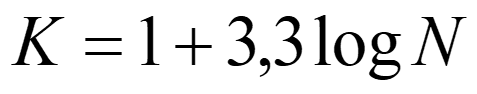
\includegraphics[scale=0.5]{figures/disfrek1}
		\end{center}
	}
	\only<3->{
		Dimana;
		\small	{

			K = Jumlah Kelas \\
			N = banyaknya frekuensi data} }
\end{frame}

\begin{frame}[c]
	\frametitle{Cara membuat distribusi frekuensi}
	\framesubtitle{Langkah 2}
	\textbf{Menentukan Interval Kelas}

	Menentukan besarnya interval kelas dilakukan dengan menggunakan rumus sebagai berikut :

	\begin{center}
		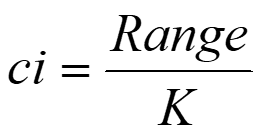
\includegraphics[scale=0.5]{figures/disfrek2}
	\end{center}

	{\small
	Dimana ;
	Range = selisih nilai tertinggi dengan nilai terendah\\
	K = jumlah interval kelas\\
	Ci  = besarnya interval kelas}
	\begin{textblock*}{2cm}(10cm,7cm) % {block width} (coords.12,8cm)
		
\includegraphics[width=2cm]{figures/cons}
	\end{textblock*}

\end{frame}

\begin{frame}[c]
	\frametitle{Cara membuat distribusi frekuensi}
	\framesubtitle{Langkah 3}

	\textbf{Memasukkan Frekuensi pada kelas-kelas}

	Setelah mengetahui banyaknya kelas yang terbentuk dan jarak antar kelas, maka dapat memasukkan data mentah (raw data ke dalam table frekuensi)
\end{frame}

{\bcb
\bodyw
\begin{frame}[c]
	\frametitle{Contoh Membuat Distribusi Frekuensi}
	\framesubtitle{data gaji per minggu SPG The Botol di Jakarta Fair }
	\begin{tabular}{llllllllll}
		60  &  33  &  85  &  52  &  65  &  77  &  84  &  65  &  57  &  74  \\
		71  &  81  &  35  &  50  &  35  &  64  &  74  &  47  &  68  &  54  \\
		80  &  41  &  61  &  91  &  55  &  73  &  59  &  53  &  45  &  77  \\
		41  &  78  &  55  &  48  &  69  &  85  &  67  &  39  &  76  &  60  \\
		94  &  66  &  98  &  66  &  73  &  42  &  65  &  94  &  89  &  88  \\
	\end{tabular}
\end{frame}}


\begin{frame}[c]
	\frametitle{}
	\framesubtitle{Contoh Membuat Distribusi Frekuensi}
	\only<1->{
		{\Large
				Jumlah data adalah 50 (n=50)

				Data yang  paling kecil adalah 33 dan yang paling besar adalah 98}}


	\only<2->{
		\textbf{Menentukan Jumlah kelas}

		\begin{figure}
			\begin{center}
				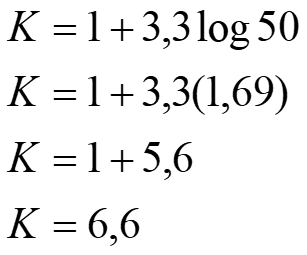
\includegraphics[scale=0.5]{figures/disfrek3}
			\end{center}
		\end{figure}

		Dibulatkan menjadi \textcolor{blue}{7 kelas}
	}
	\begin{textblock*}{2cm}(10cm,7cm) % {block width} (coords.12,8cm)
		
\includegraphics[width=2cm]{figures/cons}
	\end{textblock*}

\end{frame}

\begin{frame}[c]
	\textbf{Menentukan interval kelas:}
	\begin{figure}
		\begin{center}
			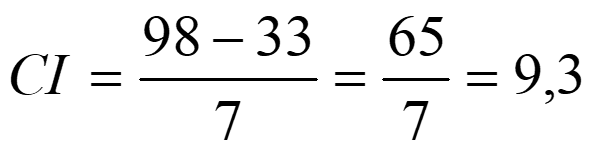
\includegraphics[scale=0.5]{figures/disfrek4}
		\end{center}
	\end{figure}
	Dibulatkan menjadi \textcolor{blue}{10 kelas}

\end{frame}

\begin{frame}[c]
	\frametitle{Cara membuat Distribusi Frekuensi}
	\framesubtitle{Pengelompokan data}
	\begin{table}[htb]
		\caption{Gaji karyawan}
		\begin{tabular}{ll}
			\hline
			Tahun  &  Pendapatan Nasional  \\
			\hline
			30-39  &  4  \\
			40-49  &  6  \\
			50-59  &  8  \\
			60-69  &  12  \\
			70-79  &  9  \\
			80-89  &  7  \\
			90-99  &  4  \\
			\hline
		\end{tabular}
	\end{table}
\end{frame}


\begin{frame}[c]
	\frametitle{Cara membuat Distribusi Frekuensi}
	\framesubtitle{Penyajian data}
	\begin{figure}
		\begin{center}
			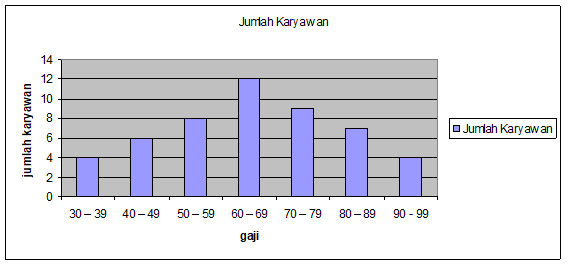
\includegraphics[scale=0.6]{figures/graph1}
		\end{center}
	\end{figure}
\end{frame}

\begin{frame}[c]
	\frametitle{Cara membuat Distribusi Frekuensi}
	\framesubtitle{Penyajian data}
	\begin{figure}
		\begin{center}
			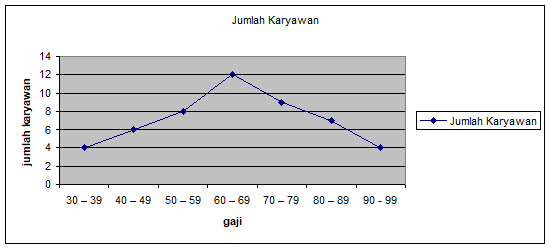
\includegraphics[scale=0.6]{figures/graph2}
		\end{center}
	\end{figure}
\end{frame}


\begin{frame}[c]
	\frametitle{Cara membuat Distribusi Frekuensi}
	\framesubtitle{Penyajian data}
	Kurva ogive
	\begin{figure}
		\begin{center}
			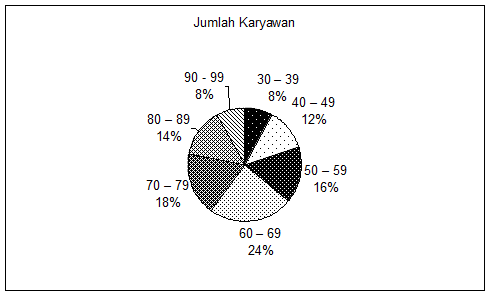
\includegraphics[scale=0.6]{figures/graph3}
		\end{center}
	\end{figure}
\end{frame}

\end{document}
